\chapter{Implementation}
\label{implementation}
The chapter \textit{\nameref{implementation}} consists of the three sections \textit{\nameref{sysarchitecture}}, \textit{\nameref{technologies}} and \textit{\nameref{implementationconsequences}}. \textit{\nameref{sysarchitecture}} defines the architecture of the current implementation of the CliniScale back end and mobile application. \textit{\nameref{technologies}} presents the frameworks and libraries used in the implementation. The third section, \textit{\nameref{implementationconsequences}}, proposes guidance in how to implement identified controls.

\section{CliniScale System Architecture}
\label{sysarchitecture}
This section presents the system architecture of the current implementation of the CliniScale project, both the back end services and the mobile application.
\newline
The back end consists of the microservices \textit{Gateway} and \textit{Study Configurator}.\\
The \textit{Gateway}, implemented using the Spring Netflix Zuul framework, provides routing and load balance functionality. It routes incoming \textit{REST} requests to the \textit{Study Configurator} microservice. It also implements basic user authentication by using \textit{JSON Web Token}.\\
The \textit{Study Configurator} microservice reacts to incoming \textit{REST} requests by gathering and processing the asked information in case of a successful authentication.\\
Both the gateway and the \textit{Study Configurator} are connected to a \textit{MySQL}\footnote{MySQL: \url{https://www.mysql.com/}. (Online; last accessed:  November 18, 2019)} database, where information is stored and retrieved on demand.\\
\newline
The Android mobile application is coded in \textit{Kotlin}, the official supported programming language for development for Android\footnote{Android: \url{https://www.android.com/}. (Online; last accessed:  November 18, 2019)}.\\
\newline
Figure \ref{fig:csarchitecture} presents a model of the CliniScale system architecture.

\begin{figure}
  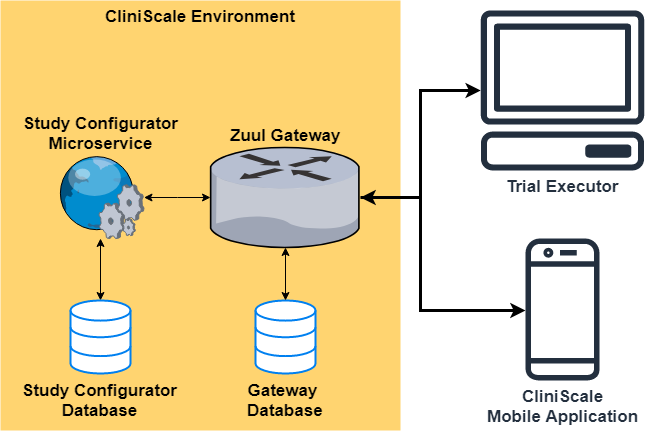
\includegraphics[width=\linewidth]{images/cs-architecture.png}
  \caption{CliniScale System Architecture}
  \label{fig:csarchitecture}
\end{figure}


\section{Technologies}
\label{technologies}

The section \textit{Technologies} presents the frameworks and libraries used in the implementation of the CliniScale back end and the CliniScale mobile application. Following the frameworks and libraries relevant to this thesis are presented:\\
\newline
\paragraph{Spring Security}\footnote{Spring Security: \url{https://spring.io/projects/spring-security}. (Online; last accessed:  November 18, 2019)} Spring security is a framework that focuses on offering highly customizable authentication, authorization and other security features to Java\footnote{Java: \url{https://www.java.com/en/}. (Online; last accessed:  November 18, 2019)} applications. It supports a wide range of security features and functions and offers a high customizability.

\paragraph{Logback}\footnote{Logback: \url{http://logback.qos.ch/}. (Online; last accessed:  November 18, 2019)} This logging framework was created as a successor to the \textit{log4j}\footnote{Log4j: \url{https://logging.apache.org/log4j/2.x/}. (Online; last accessed:  November 18, 2019)} project. \textit{Logback} improves the implementation of \textit{log4j} with a number of improvements, such as faster implementation, extended tests or an improved documentation.

\paragraph{Zuul}\footnote{Spring Zuul Documentation: \url{https://cloud.spring.io/spring-cloud-netflix/multi/multi__router_and_filter_zuul.html}. (Online; last accessed:  November 18, 2019)} Spring Zuul is a JVM-based router and server-side load balancer developed by Netflix. It is used as gateway in the CliniScale back end. It routes incoming requests to the appropriate micro-services. The Spring integration is part of the Spring Cloud Netflix framework\footnote{Spring Cloud Netflix: \url{https://spring.io/projects/spring-cloud-netflix}. (Online; last accessed:  November 18, 2019)}. Among the features, the following are of interest for this thesis: authentication and security. Zuul supports the use of the OAuth2 protocol\footnote{OAuth2: \url{https://oauth.net/2/}. (Online; last accessed:  November 18, 2019)}, which is an industry standard authentication protocol.

\paragraph{Spring Boot}\footnote{Spring Boot: \url{https://spring.io/projects/spring-boot}. (Online; last accessed:  November 18, 2019)} This is a framework used to create microservices in Java. It provides the user with many features to build standalone and production ready spring applications.

\paragraph{Kotlin}\footnote{Kotlin: \url{https://kotlinlang.org/}. (Online; last accessed:  November 18, 2019)} Kotlin is a programming language introduced by JetBrains\footnote{JetBrains: \url{https://www.jetbrains.com/}. (Online; last accessed:  November 18, 2019)}. Kotlin is designed to fully interoperate with the Java\footnote{Android: \url{https://www.android.com/}. (Online; last accessed:  November 18, 2019)} and is compatible with all standard libraries of Android.

\section{Consequences for the Implementation}
\label{implementationconsequences}

This section defines basic implementation and configuration principles to implement the identified controls of the security risk assessment into the system architecture of the CliniScale project. Its subsections represent the ten categories used by the Microsoft Threat Modeling Tool to categorize controls. In each category, basic principles are defined suggesting on how to best implement controls identified in the process of the security risk assessment and which part of the CliniScale system architecture are concerned. Microsoft suggests prioritizing the categories "Input Validation", "Authentication" and "Authorization". 


\subsection{Auditing and Logging}
Auditing and logging present a set of security controls mainly concerned with mitigating threats targeting the security property of "Accountability".
\newline
In the process of the security risk assessment, seven control classes have been identified in this category.
\begin{itemize}
    \item CC.1.1: Ensure that auditing and logging is enforced on Web API
    \item CC.1.2: Ensure that log rotation and separation are in place
    \item CC.1.3: Ensure that the application does not log sensitive user data
    \item CC.1.4: Ensure that Audit and Log Files have Restricted Access
    \item CC.1.5: Ensure that User Management Events are Logged
    \item CC.1.6: Ensure that auditing and logging is enforced on the application
    \item CC.1.7: Ensure that the system has inbuilt defences against misuse
\end{itemize}

Controls of this category affect both the CliniScale environment and the mobile application. 
These controls can be divided into two areas of application: Auditing/Logging management and Auditing/Logging usage.

\paragraph{Auditing/Logging Management} This category consists of controls regarding the implementation, configuration and management of auditing and logging mechanisms. The control classes "CC.1.1", "CC.1.2", "CC.1.4" and "CC.1.6" are meant with it. "CC.1.1" and "CC.1.6" advocate to implement auditing and logging in the application, be it the back end micro-services or the mobile application. "CC.1.2" recommends using two processes: log rotation and log separation. Log rotation describes the process of automatically naming, archiving and compressing logs based on different metrics such as time intervals or size of the log. Usually the goal is to create an automated system that archives logs in a set time interval to ease log management. \textit{Logback}, the logging framework used in the CliniScale system, supports log rotation offering the configuration of \textit{Appenders}\footnote{Logback Appenders: \url{http://logback.qos.ch/manual/appenders.html}. (Online; last accessed:  November 18, 2019)}. Log separation describes the process of sorting log files on a different partition as where the OS/application is running in order to avert a Denial of service attack. \textit{Logback} supports the configuration of the folder in which logs get stored in the process of log rotation. "CC.1.4" advocates to limit access to stored log files. It is recommended that applications have write-only access and operators and support personnel have read-only access. Only administrators should have full access to the log files.\\

\paragraph{Auditing/Logging Usage} Controls of this category describe principles on what to, or specifically not to, log. The control classes "CC.1.3", "CC.1.5" and "CC.1.7" advocate on which events should, or should not, be logged.  "CC.1.3" advocates to not log sensitive data, like user credentials, health information or encryption keys. Logging these kind of data opens additional ways for an adversary to obtain the data. "CC.1.5" proposes to log all user management events, such as successful and failed logins, password resets or user registrations. This enables to detect and react to suspicious behavior. "CC.1.7" advises logging security exceptions to enable detection of suspicious activities. It is recommended to have security exceptions for issues such as input validation, file upload violations or brute forcing of user logins. If such an exception occurs, further measurements, depending on the exception, should prevent further abuse. If an adversary tries to brute force user credentials, the account should be suspended for a period of time and a notification to the user should be send.

\subsection{Authentication}
Proving an entities identity is crucial for the security of an application. Controls of this control class ensure the integrity of the name giving security goal.\\
This category consists of eight control classes:
\begin{itemize}
    \item CC.2.1: Consider using a standard authentication mechanism to authenticate to Web Application
    \item CC.2.2: Enable step up or adaptive authentication
    \item CC.2.3: Ensure that administrative interfaces are appropriately locked down
    \item CC.2.4: Implement forgot password functionalities securely
    \item CC.2.5: Ensure that password and account policy are implemented
    \item CC.2.6: Implement controls to prevent username enumeration
    \item CC.2.7: Ensure that standard authentication techniques are used to secure Web APIs
    \item CC.2.8: Use ADAL libraries to manage token requests from OAuth2 clients to AAD (or on-premises AD)
\end{itemize}

The controls mainly concern the back end of the CliniScale project. "CC.2.1" and "CC.2.7" recommend using standard authentication mechanisms, such as credentials consisting of username and password, to access CliniScale services. "CC.2.2" advocates the use of mechanisms such as two-factor authentication or the usage of One-Time-Passwords send via mail or SMS to further authenticate an user when logging in, accessing sensitive information or making critical changes to an account such as changing the password. "CC.2.3" requires administrative interfaces to be secured in an advanced manner by requiring two-factor authentication or setting it up to only be accessible from specific IP ranges. "CC.2.4" and "CC.2.5" advocate on password policies and the handling of password retrieval. Per default, a strong password policy should be implemented to prevent dictionary based or brute force attacks. Measures should be implemented to force users to create complex passwords, such as minimum password length, usage of special characters and the use of two-factor authentication. A secure password policy should also implement measures to protect user accounts from adversaries. A soft lock-out, disabling the account for a set time-frame after repeatedly entering the wrong password, protects against brute force attacks on user accounts. A hard lock-out can help if an account is performing malicious activities. Additionally, verify that standard passwords of software or hardware are changed after installation. To generate passwords, a password generator based on a proven random number generator should be used. Password recovery should be implemented using two-factor authentication whenever possible. To implement the control class "CC.2.6" it is required to set up a generalized error message to prevent adversaries from obtaining additional information. "CC.2.8" is a Microsoft specific control class that does not apply to the CliniScale project.

\subsection{Authorization}
Authorization ensures that services and data is only accessed by parties with the rights to do so. Six control classes have been identified in this category:

\begin{itemize}
    \item CC.3.1: Enforce sequential step order when processing business logic flows
    \item CC.3.2: Ensure that proper authorization is in place and principle of least privileges is followed
    \item CC.3.3: Business logic and resource access authorization decisions should not be based on incoming request parameters
    \item CC.3.4: Ensure that content and resources are not enumerable or accessible via forceful browsing
    \item CC.3.5: Implement implicit jailbreak or rooting detection
    \item CC.3.6: Implement proper authorization mechanism in ASP.NET Web API
\end{itemize}

These controls concern both the back end and the mobile application. "CC.3.1" advocates to implement mechanism to prevent automatic exploitation of offered services, for example by running a bot, by an adversary to gather as much information as possible. These mechanisms could be logic that checks for processes to be run in sequential order, without skipping single steps or passing steps in a time that no genuine human being could. "CC.3.4" goes hand in hand with this, suggesting implementing logic to prevent acquiring large amounts of data by enumerating requests, e.g. by implementing CAPTCHA controls or randomized identifiers. "CC.3.2" advocates to follow the principle of least privileges. This principle requires users to have no rights at all per default. Specific user roles get exactly the privileges they need so the user can perform the work he is intended to be able to perform. A user whose job is to manage the database does not need the rights to install new software. Same goes for processes, if a normal user does not need access to specific data, he should not have the right to do it. Using the Spring Security framework, user roles and privileges can be defined to implement this principle. "CC.3.3" advocates to perform all user access restriction checks server-side. To do this, the UserID could be stored in the session cookie and checked on server-side whenever a user wants to access data or services. The control class "CC.3.5" recommends implementing jailbreak or rooting detection to safeguard the applications configuration. These mechanisms should be implemented to check on startup of the application and deny execution of the application in case of a jailbreaked or rooted mobile device. "CC.3.6" advocates to implement authorization mechanism in the Web API. Spring Security offers solutions to this problem by supporting roles and privileges which can be assigned to user classes.

\subsection{Communication Security}
The category "Communication Security" ensures all communication is done in a as secure as possible manner. The four control classes recommend using proven secure communication standards in order to ensure the security and privacy of the communication channels.

\begin{itemize}
    \item CC.4.1: Verify X.509 certificates used to authenticate SSL, TLS, and DTLS connections
    \item CC.4.2: Enable HTTP Strict Transport Security (HSTS)
    \item CC.4.3: Implement Certificate Pinning
    \item CC.4.4: Force all traffic to Web APIs over HTTPS connection 
\end{itemize}

Implementation of these control classes concerns the CliniScale back end. "CC.4.2" and "CC.4.4" recommend using the Hypertext Transfer Protocol Secure (HTTPS) protocol for every connection. The HTTPS protocol is an extension of the HTTP protocol, encrypting it using Transport Layer Security (TLS), or its predecessor, Secure Socket Layer (SSL). Using HTTPS offers authentication of the website and integrity and privacy of the content of the communication. When using two-way TLS, or TLS with client authentication, a client certificate is also involved hardening the authentication process. By enabling HSTS, all communication to and from the server is forced to use HTTPS. HTTPS offers protection against Man-in-the-middle attacks, eavesdropping and tampering of the communication. Spring Security supports the use of most basic TLS versions. The BSI TR-02102-2 suggests using the TLS version 1.2 or 1.3 with enabled Perfect Forward Security (PFS). PFS is a feature protecting past sessions against future compromise of secret keys by generating a unique session key for every session. Any cipher-suite and configuration recommended by the TR-02102-2 can be used to ensure a security level that holds up till at least the year 2025. "CC.4.1" advocates to verify the X.509 certificate of an SSL, TLS or DTLS connection. X.509 is a public key infrastructure standard that can be used to verify the identity of a user and that a public key is contained within a certificate signed by a trusted certificate authority. These certificates are routinely used to verify the identity of an entity within the internet. In the process of verifying a certificate, many attributes can be audited, e.g. domain name, trust chains or key lengths. In order to provide a high level of trust, as many attributes as possible should be verified. "CC.4.3" advises to implement certificate pinning in a mobile application. Certificate pinning describes the process of associating a host with their expected X.509 certificate or public key. If an attacker tries to start a Man-in-the-middle attack, the certificate or public key would differ from the saved one.

\subsection{Configuration Management}
Configuration management refers to the management of configurations for an information system with the goal of enabling security managing risk. It consists of ten control classes:

\begin{itemize}
    \item CC.5.1: Implement Content Security Policy (CSP), and disable inline javascript
    \item CC.5.2: Enable browser's XSS filter
    \item CC.5.3: ASP.NET applications must disable tracing and debugging prior to deployment
    \item CC.5.4: Ensure that only trusted origins are allowed if CORS is enabled on ASP.NET Web Applications
    \item CC.5.5: Enable ValidateRequest attribute on ASP.NET Pages
    \item CC.5.6: Use locally-hosted latest versions of JavaScript libraries
    \item CC.5.7: Disable automatic MIME sniffing
    \item CC.5.8: Encrypt sections of Web API's configuration files that contain sensitive data
    \item CC.5.9: Ensure that authenticated ASP.NET pages incorporate UI Redressing or click-jacking defenses
    \item CC.5.10: Access third party javascripts from trusted sources only
\end{itemize}

These control classes are implemented in the back end. "CC.5.1" suggests implementing CSP to protect against different sort of attacks, such as XSS, data exfiltration or click-jacking. Spring Security supports to set the needed flag in the HTTP request\footnote{Spring Security Headers: \url{https://docs.spring.io/spring-security/site/docs/3.2.0.CI-SNAPSHOT/reference/html/headers.html}. (Online; last accessed:  November 18, 2019)}. "CC.5.2" advocates to enable a user’s browser XSS filter to protect against cross site scripting attacks. Spring Security supports setting this header similar to enabling CPS. "CC.5.3" refers to technology no used in the CliniScale project, nonetheless the recommendation stays true. Disabling debugging modes is essential when configuring live versions of the system. "CC.5.4" recommends to only allow trusted origins when using Cross-Origin Resource Sharing (CORS). Setting this option is supported by the Spring Security framework. "CC.5.5" advocates to enable request validation to prevent adversaries from being able to execute specific script-injection attacks. The Spring Data frameworks supports this feature by implementing the Validator interface \footnote{Spring Data Rest Validator: \url{https://docs.spring.io/spring-data/rest/docs/current/reference/html/\#validation}. (Online; last accessed:  November 18, 2019)}. "CC.5.6" and "CC.5.10" recommend to only use up-to-date javascript libraries and reference them only from trusted origins and, when possible, over a HTTPS secured connection. "CC.5.7" advises to disable content sniffing for web browsers. This option can be set using the Spring Security framework in a similar way to enabling CSP and XSS filters. "CC.5.8" recommends encrypting sensitive data, such as usernames and passwords, in configuration files. The Spring Boot framework can be used together with the tool Jasypt (Java Simplified Encryption) to encrypt sensitive data in configuration files\footnote{Spring Boot Configuration with Jasypt: \url{https://www.baeldung.com/spring-boot-jasypt}. (Online; last accessed:  November 18, 2019)}. "CC.5.9" recommends preventing click-jacking attacks. Spring Security enables this feature per default. In case the option has to be set manually, the process is similar to setting the other HTTP request headers.

\subsection{Cryptography}
Control classes of this category give recommendations on which protocols to use to perform cryptography and how they should be configured. There are six control classes:

\begin{itemize}
    \item CC.6.1: Use only approved symmetric block ciphers and key lengths
    \item CC.6.2: Use approved block cipher modes and initialization vectors for symmetric ciphers
    \item CC.6.3: Use approved asymmetric algorithms, key lengths, and padding
    \item CC.6.4: Use approved random number generators
    \item CC.6.5: Do not use symmetric stream ciphers
    \item CC.6.6: Use approved MAC/HMAC/keyed hash algorithms
\end{itemize}

The implementation of these control classes applies to both the back end and the mobile application. The BSI TR-02102-1 and TR-02102-2 give state of the art recommendations on which protocols, cipher-suites and configurations to use. For all of these control classes, these documents provide valuable guidance. The Spring Security framework offers support for most protocols, cipher-suites and configurations.\\
\newline
To ensure the secure storage of security keys on mobile devices, a Trusted Execution Environment (TEE)\footnote{Trusted Execution Environment: \url{https://www.trustonic.com/news/technology/what-is-a-trusted-execution-environment-tee/}. (Online; last accessed:  November 18, 2019)} should be used. A TEE is a secure area of the main processor guaranteeing data and code loaded into it to be secure regarding confidentiality and integrity. Android 4.3 (API level 18)\footnote{Android 4.3 Jelly Bean: \url{https://www.android.com/intl/de_de/versions/jelly-bean-4-3/}. (Online; last accessed:  November 18, 2019)} and higher support the implementation of the Android Keystore\footnote{Android Keystore: \url{https://developer.android.com/training/articles/keystore}. (Online; last accessed:  November 18, 2019)}. Android Keystore supports most of the cryptographic algorithms listed in the technical guidelines of the BSI.

\subsection{Exception Management}
Exception Management describes handling of software failures, be it forced or accidental, in a secure manner. The five control classes of this category are the following:

\begin{itemize}
    \item CC.7.1: Ensure that proper exception handling is done in ASP.NET Web API
    \item CC.7.2: Do not expose security details in error messages
    \item CC.7.3: Implement Default error handling page
    \item CC.7.4: Set Deployment Method to Retail in IIS
    \item CC.7.5: Exceptions should fail safely
\end{itemize}

The implementation of these controls concerns the back end and the mobile application. Most important of these control classes is "CC.7.3". It advises to implement a default error handling page which does not divulges any, possible critical to security, information. Possible failure trigger can be logged server-side but should never be shown to a user to prevent possible adversaries from obtaining information they should not have access to. Spring Boot supports creating and using custom error pages. "CC.7.1" proposes to implement proper exception handling in Web APIs. Per default, the default error handling page described before is what should be shown to a user in case of any exception. "CC.7.2" advocates to omit sensitive data, such as server names, procedures, etc., from error messages to prevent an adversary from obtaining any additional information. In case of an exception, security details, such as the stack trace or details of failed procedures, should be logged. "CC.7.4" recommends setting possible deployment methods to retail when an application is deployed in a live environment. Different settings, for example debug mode, may lead to information disclosure. "CC.7.5" advocates to implement a proper exception handling throughout the entire code base. The Spring frameworks offer a lot of functionality on the topic of exception handling\footnote{Spring Exception Handling: \url{https://spring.io/blog/2013/11/01/exception-handling-in-spring-mvc}. (Online; last accessed:  November 18, 2019)}.

\subsection{Input Validation}
This category consists of control classes defining how to filter, scrub or reject the input to the application before further processing. This category consists of 13 control classes:


\begin{itemize}
    \item CC.8.1: Ensure that each page that could contain user controllable content opts out of automatic MIME sniffing
    \item CC.8.2: Ensure appropriate controls are in place when accepting files from users
    \item CC.8.3: Ensure that type-safe parameters are used in Web Application for data access
    \item CC.8.4: Encode untrusted web output prior to rendering
    \item CC.8.5: Perform input validation and filtering on all string type Model properties
    \item CC.8.6: Do not assign DOM elements to sinks that do not have inbuilt encoding
    \item CC.8.7: Validate all redirects within the application are closed or done safely
    \item CC.8.8: Implement input validation on all string type parameters accepted by Controller methods
    \item CC.8.9: Avoid using Html.Raw in Razor views
    \item CC.8.10: Ensure that model validation is done on Web API methods
    \item CC.8.11: Implement input validation on all string type parameters accepted by Web API methods
    \item CC.8.12: Ensure that type-safe parameters are used in Web API for data access
    \item CC.8.13: Sanitization should be applied on form fields that accept all characters e.g, rich text editor
\end{itemize}

The implementation of control classes of this category concerns the back end. The category can be further split into two sub-categories:
\paragraph{User Input Validation} Control classes of this category focus on validating a given users input. "CC.8.5", "CC.8.8", "CC.8.10" and "CC.8.11" all recommend input validation on any string type parameter in the Web API, controller classes or model properties. A whitelist validation strategy is recommended, meaning that per default all inputs are invalid and only expected values are accepted by using regular expressions. Spring frameworks support various ways to perform input validation further described in the documentation\footnote{Spring Validation, Data Binding, and Type Conversion: \url{https://docs.spring.io/spring/docs/4.1.x/spring-framework-reference/html/validation.html}. (Online; last accessed:  November 18, 2019)}.
"CC.8.2" advocates to implement measures to user file upload. Many attacks process is to somehow get code into the system attacked and then execute it. A user file upload can help the attacker perform the first step. Many possible measures exist to prevent this problem: File extension checks, maximum file size limit, validating naming conventions, scan the file with an anti-virus or save the file on a non-system drive. "CC.8.3" and "CC.8.12" recommend using type safe parameters to prevent injection attacks. Parameters can be used to enforce length and type constraints on input data. Type safe parameters also prevent code execution, as the database treats them as literal values and not as executable code. \\

\paragraph{Input Validation Configuration} Control classes of this category prevent abuse of user input by disabling options per configuration. "CC.8.1" recommends, similar to "CC.5.1", to disable automated MIME sniffing by setting the HTTP header "X-Content-Type-Options:nosniff". Spring Security supports setting this header, as described in "CC.5.1". "CC.8.4" advocates to encode untrusted web output to prevent cross-site scripting attacks. To implement this control class, it is recommended to perform input validation and encoding of user input before it is rendering. "CC.8.6" recommends to not assign untrusted input to DOM elements, since many javascript functions do not perform encoding by default. "CC.8.7" advocates to whitelist possible redirections to user-supplied locations. This prevents adversaries from possible stealing a user’s logon token to services like Facebook/OAuth/OpenID. "CC.8.9" advocates to not use any functions that may bypass automatic encoding protection, like the HtmlHelper.Raw method, that return not HTML encoded code. "CC.8.13" recommends performing sanitization on all form fields that accept all characters. Sanitization cleans HTML fragments and prevents cross-site scripting attacks. If proper input validation and output encoding measures are implemented, there is no need for sanitization.

\subsection{Sensitive Data}
The category "Sensitive Data" consists of control classes securing name giving data by protecting it in memory, over the network or on storage in browser or mobile application. There are seven control classes in this category:

\begin{itemize}
    \item CC.9.1: Ensure that sensitive content is not cached on the browser
    \item CC.9.2: Encrypt sections of Web App's configuration files that contain sensitive data
    \item CC.9.3: Explicitly disable the autocomplete HTML attribute in sensitive forms and inputs
    \item CC.9.4: Ensure that sensitive data displayed on the user screen is masked
    \item CC.9.5: Ensure that sensitive data relevant to Web API is not stored in browser's storage
    \item CC.9.6: Encrypt sensitive or PII data written to phones local storage
    \item CC.9.7: Obfuscate generated binaries before distributing to end users
\end{itemize}

Implementation of these control classes concerns both the back end and the mobile application. "CC.9.1" and "CC.9.5" recommend to not cache any sensitive data in the browser. Cached data, such as username, health data or personal details, can be accessible even after the user logs off. Especially on shared computers these can lead to grave information disclosure. To prevent a browser from caching data, a response header called "Cache-Control" can be set to "no-cache". The Spring Security framework supports setting this option by using the CacheControl class\footnote{Spring Security CacheControl: \url{https://docs.spring.io/spring-framework/docs/current/javadoc-api/org/springframework/http/CacheControl.html}. (Online; last accessed:  November 18, 2019)}. "CC.9.2" recommends encrypting sensitive data in configuration files, such as server addresses and passwords, to prevent adversaries of gaining access to the data. See "CC.5.8" for an explanation on the implementation. "CC.9.3" advocates to disable autocomplete on sensitive forms and inputs, such as username/password. By default, autocomplete is on. To disable autocomplete, the attribute "autocomplete" should be se to "off" either on the entire form or single input fields. "CC.9.4" recommends masking sensitive data displayed for a user, preventing adversaries from accessing the data. Masking data has to be taken care off when the data is accepted as input, e.g. by setting the HTML attribute "input type" to "password", and when displayed on the screen, e.g. by displaying only the last digits of a sensitive number such as credit card number. "CC.9.6" recommends encrypting sensitive information that is saved on the mobile device's file system. This prevents attackers from accessing the data, e.g. when they root the phone and can read out the local file storage. "CC.9.7" recommends obfuscating generated binaries, e.g. apk files for Android mobile devices, to prevent adversaries from reverse engineering the assemblies. Tools, such as ProGuard\footnote{ProGuard: \url{https://www.guardsquare.com/en/products/proguard}. (Online; last accessed:  November 18, 2019)}, can be used for this purpose.

\subsection{Session Management}
Control classes of this category secure user sessions between the user and the web application. The category consists of five control classes:
\begin{itemize}
    \item CC.10.1: Applications available over HTTPS must use secure cookies
    \item CC.10.2: All http based application should specify http only for cookie definition
    \item CC.10.3: Mitigate against Cross-Site Request Forgery (CSRF) attacks on ASP.NET web pages
    \item CC.10.4: Set up session for inactivity lifetime
    \item CC.10.5: Implement proper logout from the application
\end{itemize}

Implementation of these control classes happens in the back end. "CC.10.1" recommends using secure cookies on connections using the HTTPS protocol. Secure cookies are cookies with the "secure" attribute set and are only available when using HTTPS. The Spring Security framework supports setting the "secure" attribute\footnote{Control the Session with Spring Security: \url{https://www.baeldung.com/spring-security-session}. Last access: (Online; last accessed:  November 18, 2019)}. "CC.10.2" recommends making cookies from HTTP based applications unable to be accessible by script by setting the "httpOnly" attribute. Implementation of this attribute is similar to the "secure" attribute presented in "CC.10.1". "CC.10.3" advocates to implement measures preventing CSRF attacks. Spring Security has a build in measure against this kind of attacks implementing the Token Synchronizer Pattern\footnote{Spring Security CSRF: \url{https://docs.spring.io/spring-security/site/docs/3.2.0.CI-SNAPSHOT/reference/html/csrf.html}. (Online; last accessed:  November 18, 2019)}. "CC.10.4" recommends implementing a session timeout as a measure to prevent adversaries from gaining access to an users account who has not logged off. Spring Security supports implementation of a custom session timeout timer\footnote{Control the Session with Spring Security: \url{https://www.baeldung.com/spring-security-session}. (Online; last accessed:  November 18, 2019)}. "CC.10.5" recommends destroying a user's session on user log out and reset and nullify the session cookie and authentication cookie values. The Spring Security framework offers the needed functionality\footnote{Spring Security Logout: \url{https://www.baeldung.com/spring-security-logout}. (Online; last accessed:  November 18, 2019)}.\\





